\documentclass[a4paper,12pt]{article}
\usepackage[utf8]{inputenc}
\usepackage{hyperref}
\usepackage{graphicx}
\usepackage{float}
\graphicspath{ {images/} }

\begin{document}

\begin{titlepage}

\newcommand{\HRule}{\rule{\linewidth}{0.5mm}} % Defines a new command for the horizontal lines, change thickness here

\center % Center everything on the page
 
%----------------------------------------------------------------------------------------
%-	HEADING SECTIONS
%----------------------------------------------------------------------------------------

\textsc{\LARGE University of Pretoria}\\[1.5cm]
\textsc{\Large COS 301 - Software Engineering}\\[0.5cm]
\textsc{\large The Savage Ru's}\\[0.5cm]

%----------------------------------------------------------------------------------------
%-	TITLE SECTION
%----------------------------------------------------------------------------------------

\HRule \\[0.4cm]
{ \huge \bfseries User Manual}\\ % Title of your document
\HRule \\[1.5cm]
 
%----------------------------------------------------------------------------------------
%-	AUTHOR SECTION
%----------------------------------------------------------------------------------------

\begin{minipage}{0.4\textwidth}
\begin{flushleft} \large
\emph{Author(s):}\\
Jodan \textsc{Alberts}\\ % Your name
Mark \textsc{Klingenberg}\\
Una \textsc{Rambani}\\
Ruan \textsc{Klinkert}\\
\end{flushleft}
\end{minipage}
~
\begin{minipage}{0.4\textwidth}
\begin{flushright} \large
\emph{Student number(s):} \\
14395283\\ % Student number
14020272\\
14004489\\
14022282\\

\end{flushright}

\end{minipage}\\[0.5cm]


%----------------------------------------------------------------------------------------
%-	DATE SECTION
%----------------------------------------------------------------------------------------

\centering
	
\includegraphics[width=60mm]{SavageRu.jpg}

{\large \today}\\[3cm] % Date, change the \today to a set date if you want to be precise
\newpage
\centering
	\textsc{\LARGE Epi-Use labs project}\\[0.5cm]
	\textsc{\Large VizARD}\\[0.5cm]
	\textsc{\Large User Manual version 1}\\[0.5cm]
	
\includegraphics[width=\textwidth]{images/vizard.png}
%----------------------------------------------------------------------------------------

\vfill % Fill the rest of the page with whitespace

\end{titlepage}

\newpage

\tableofcontents

\newpage

\section{Introduction}

This is the user manual for the VizARD Augmented Reality application being developed for EPI-USE Labs by The Savage Ru's.

VizARD is a mobile application which will allow a user to take a picture of tabulated data and then view, automatically generated, 3D graphs of the data projected onto the document of which the image was taken.



%%--------------------------------------INSTALLATION  ----------------------------------------
\section{Installation}
To access the VizARD application one must first install it, currently this is done by getting the VizARD apk file, and installing it onto your Android mobile phone (allow for the installation from unknown sources). In the future this application will be available through the Google Play Store.

%%-------------------------------------GETTING STARTED ----------------------------------------
\section{Configuration}
For the user VizARD is a stand alone mobile application, one simply ahs to install the apk. A server needs to be configured for the OCR, this has been done already on an Epi-Use Labs server, for a guide on the server see \url{www.github.com/tleyden/open-ocr}

\section{Getting Started}
Once the app has been installed the user simply need to click on the application named VizARD, this will bring the user into a launching screen shown in Figure 1.\\
\begin{figure}[H]
\centering
	
\includegraphics[width=50mm]{images/launch.png}
	\caption{launching screen \label{overflow}}
\end{figure}

Once the app has finished launching the user will be greeted by the landing screen.
\newpage

%%-------------------------------------LANDING SCREEN ----------------------------------------
\section{Landing Screen}
Once the app has completed loading it will then bring you to a screen that looks like Figure 2, this screen shows what the camera is looking at as well as having two buttons currently, these are the capture data circle (Figure 3) that should be familiar to users of snapchat, as well as an adjustable frame so that you can narrow down the data(Figure 4).

\begin{figure}[H]
\centering
	\includegraphics[width=50mm]{images/landing.png}
	\caption{landing screen \label{overflow}}
\end{figure}

\begin{figure}[H]
  \centering
  \begin{minipage}[b]{0.4\textwidth}
    
\includegraphics[width=50mm]{images/capture.png}
    \caption{Capture icon.}
  \end{minipage}
  \hfill
  \begin{minipage}[b]{0.4\textwidth}
    
\includegraphics[width=50mm]{images/frame.png}
    \caption{Frame.}
  \end{minipage}
\end{figure}


%%----------------------------------ON CAPTURE CLICK-----------------------------------------
\subsection{On Capture Circle click}
When a user clicks the capture data circle (Figure 3) it will choose the table that is being viewed as the target for the 3D graph that will be generated, it will also send the image to a server to allow for optical character recognition of the data to make the graph, while this is occuring the application will show a loading screen while the user waits. Once it has generated the graph the app moves to the display screen.

%--------------------------------THE FRAME---------------------------------------------------
\subsection{Frame}
The frame allows the user to select only the part of the picture they want to be used to generate the graph, this means that you are able to cut out unwanted text. The frame and be resized using two finger pinch and moved by using one finger.
%%----------------------------DISPLAY SCREEN------------------------------------------------
\section{Dispay Screen}
Once the app has completed generating the graph it will then bring you to a display screen that looks like Figure 5, this screen shows the newly generated graph that has been mapped onto the target, and two buttons, these are the edit graphs button (Figure 6), the back button (Figure 7).

\begin{figure}[H]
\centering
	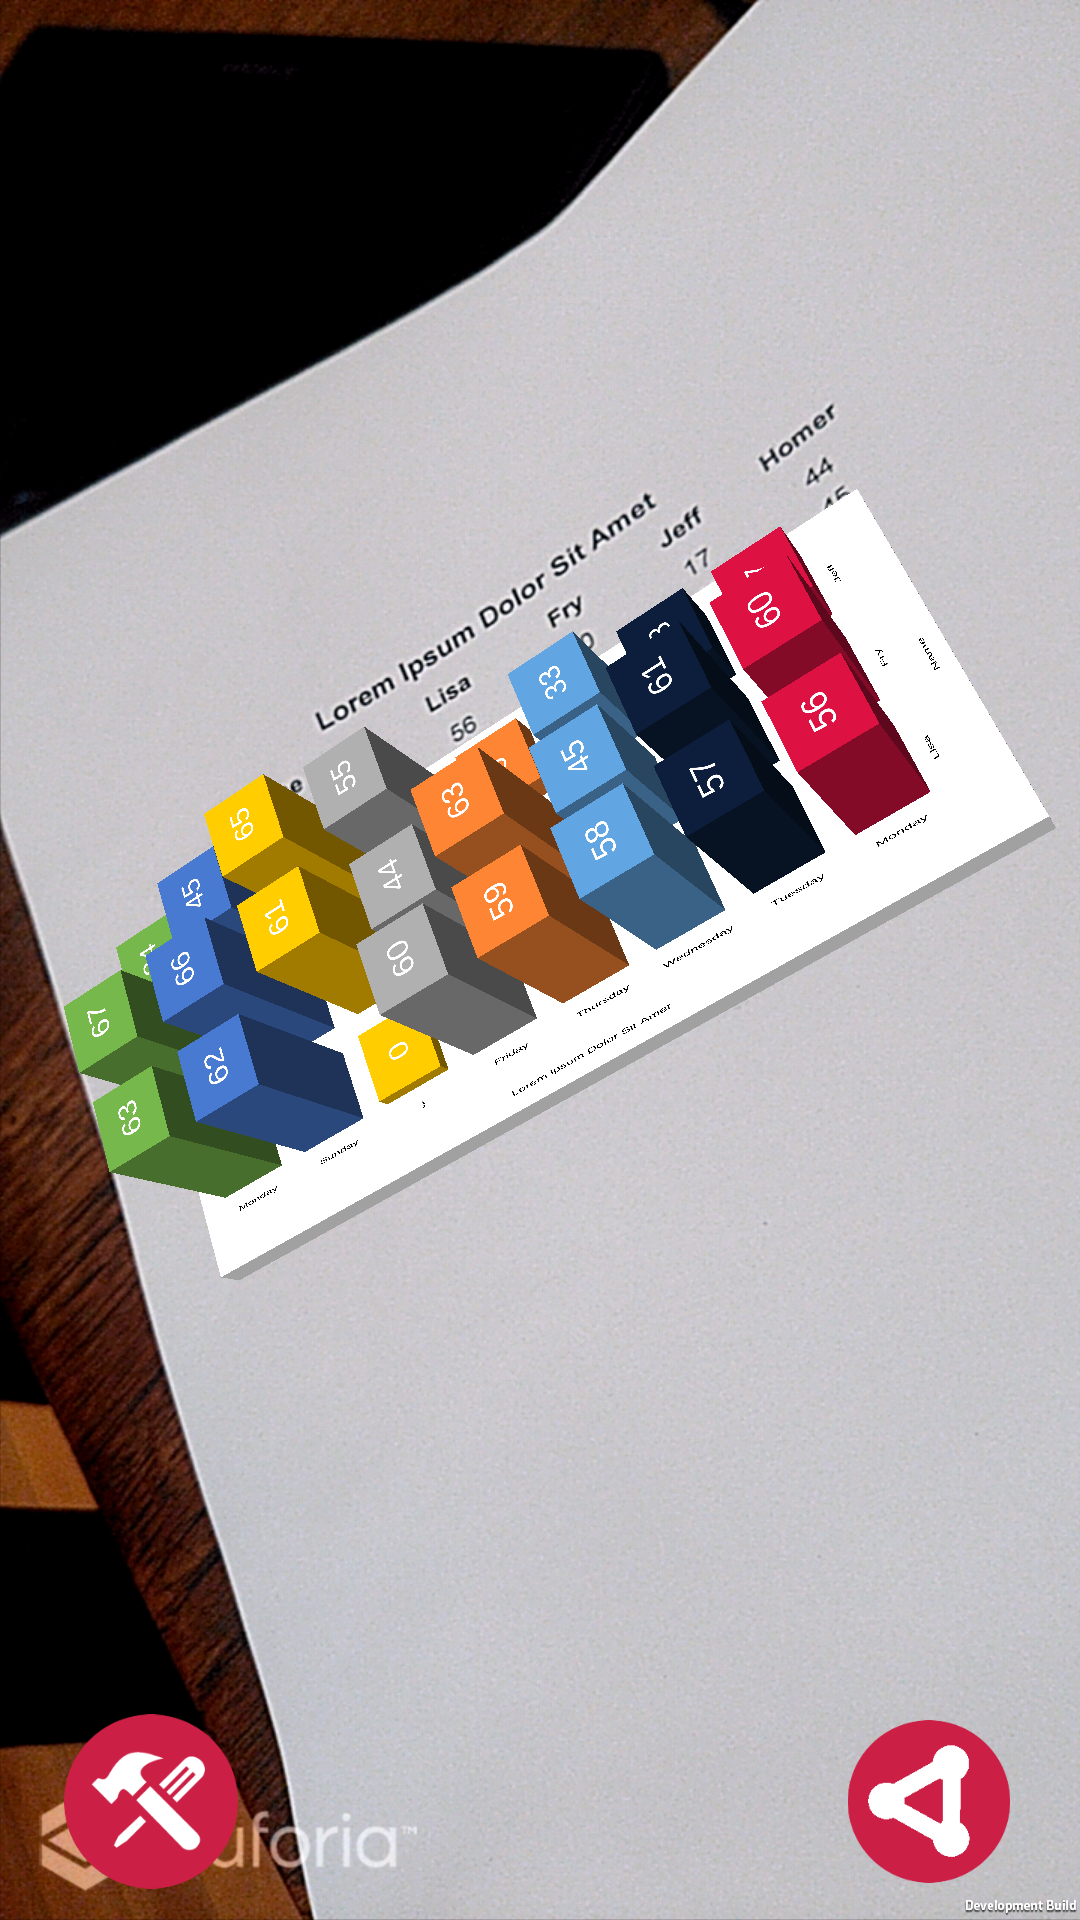
\includegraphics[width=5cm]{images/graph.png}
	\caption{display screen \label{overflow}}
\end{figure}

\begin{figure}[H]
  \centering
  \begin{minipage}[b]{0.2\textwidth}
    
\includegraphics[width=50mm]{images/editRed.png}
    \caption{Edit button}
  \end{minipage}
  \hfill
  \begin{minipage}[b]{0.2\textwidth}
    
\includegraphics[width=50mm]{images/back.png}
    \caption{Back button}
  \end{minipage}
\end{figure}
%------------------------on edit click------------------------------------
\subsection{On Edit Button click}
When the edit button is clicked a screen containing a form is shown, this form will allow the user to edit data and the graph. 

%-----------------------on back clicked----------------------------------
\subsection{Back button}
When the back button is pressed the application goes back to the capture image screen and clears all data that has been stored during the run time of the application. It then allows for a new table to be captured.
%-----------------------------form-----------------
\subsection{Form}
When the form is brought up from the edit button you see the following screen. 
\begin{figure}[H] 
\centering
    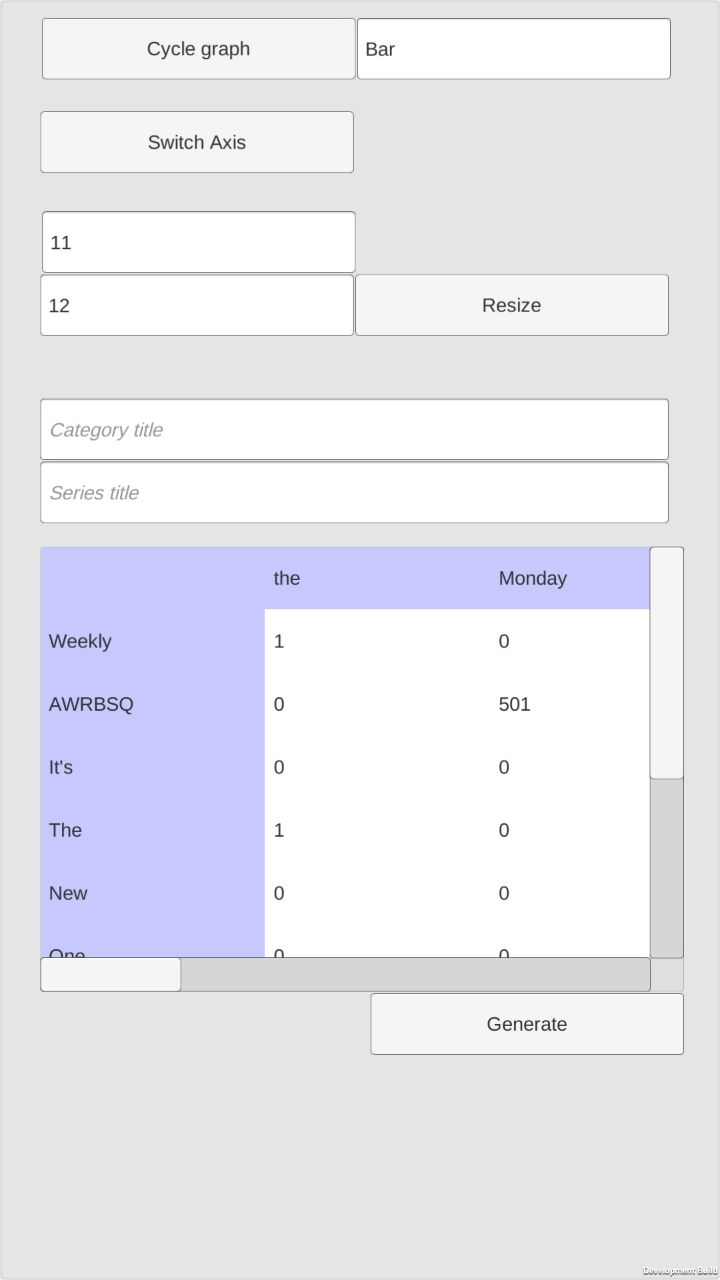
\includegraphics[width=85mm]{images/form.jpg}
    \caption{Edit form}
\end{figure}
The form contains a table that displays all the data that the OCR has read. It also allows for the switching of axis, when the switch axis button is clicked. You can cycle through graph type by pressing the "Cycle graph" button. To edit values, simply tap on the corresponding cell.

\end{document}